\newpage

%%%%%%%%%%%%%%%%%%%%%%%%%%%%%%%%%%%%%%%%%%%%%%%%%%%%%%%%%%%%%%%%%%%%%%%%%%%%%%%%%%%%%%%
%%%%%%%%%%%%%%%%%%%%%%%%%%%%%%%%%%%%%%%%%%%%%%%%%%%%%%%%%%%%%%%%%%%%%%%%%%%%%%%%%%%%%%%
%%%%%%%%%%%%%%%%%%%%%%%%%%%%%%%%%%%%%%%%%%%%%%%%%%%%%%%%%%%%%%%%%%%%%%%%%%%%%%%%%%%%%%%
\section{Regressão logística polinomial com MSE de $f_{\VECTOR{c}}(x):~\mathbb{R} \rightarrow \mathbb{R}$}

\index{Regressão!Logística polinomial $f_{\VECTOR{c}}(x):~\mathbb{R} \rightarrow \mathbb{R}$}



\begin{theorem}[Classificação de dados em $\mathbb{R}$:]\label{theo:reglogr1r1poly:1}
~\\
\noindent
\begin{minipage}{0.45\textwidth}
\centering
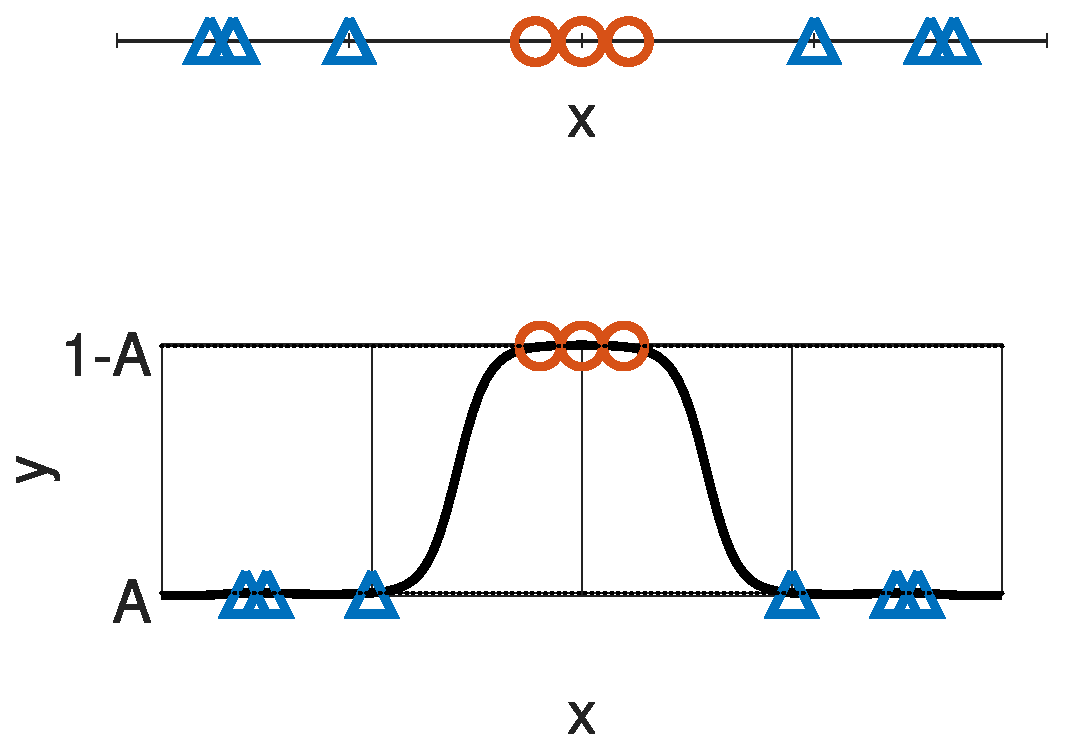
\includegraphics[width=0.95\linewidth]{chapters/classificacao/mfiles/reglogr1r1poly/reglogr1r1poly.eps} 
\end{minipage}
\begin{minipage}{0.55\textwidth}
Dados, um conjunto de $L$ dados 
$x_l$ $\in \mathbb{R}$, $1\leq l\leq L$,
%agrupados no vetor $\VECTOR{x}=[x_1,$ $x_2,$ $...,$ $x_L]^{\transpose}$ $\in \mathbb{R}^{L}$,
repartidos em dois grupos etiquetados com os símbolos $\bigtriangleup$ e $\bigcirc$,
não separáveis por um hiperplano.
Se desejamos criar um classificador mediante 
a função  $f_{\VECTOR{c}}:\mathbb{R} \rightarrow \mathbb{R}$,
com domínio $x \in \mathbb{R}$, contradomínio $y \in \mathbb{R}$ e 
parâmetros agrupados no vetor $\VECTOR{c}=[c_1$ $c_2$ $...$ $c_{M+1}]^{\transpose}\in \mathbb{R}^{M+1}$,
como definido na Eq. (\ref{eq:reglogr1r1poly:1}),
\begin{equation}\label{eq:reglogr1r1poly:1}
y\equiv f_{\VECTOR{c}}(x)= \frac{1}{1+e^{-h_{\VECTOR{c}}(x)}},
\quad h_{\VECTOR{c}}(x)=\sum\limits_{m=0}^{M}c_{m+1}x^m,
\end{equation}
ou seu equivalente: $logit(y)=h_{\VECTOR{c}}(x)$.
\end{minipage}
Podemos atribuir a cada valor $x_l$ uma etiqueta $y_l\in \{A,1-A\}$, 
onde $0<A\ll 0.5$ é escolhido por nós,
e afirmar que o vetor $\VECTOR{c}= \VECTOR{\hat{c}}$,
que minimiza o erro quadrático médio\footnote{Do inglês ``mean square error'' com siglas $MSE$.} $e(\VECTOR{c})$,
\begin{equation}\label{eq:reglogr1r1poly:1e}
e(\VECTOR{c}) =  \frac{1}{L}\sum_{l=1}^{L} w_l||h_{\VECTOR{c}}(x_l)-logit(y_l)||^2,
\end{equation}
ponderado com os pesos $w_l \in \mathbb{R}_+$ 
pode ser calculado com a Eq. (\ref{eq:reglogr1r1poly:2});
onde a matriz  $\MATRIX{W}=\funcdiag \left( \left[w_1,~ w_2,~ ...,~ w_L \right]^{\transpose} \right) $;
%e $\VECTOR{x}^m$ representa uma potencia $m$ de cada elemento;
\begin{equation}\label{eq:reglogr1r1poly:2}
\VECTOR{\hat{c}} =  \left[ \MATRIX{A}^{\transpose} \MATRIX{W}\MATRIX{A}\right]^{-1} \MATRIX{A}^{\transpose} \MATRIX{W}\VECTOR{z},
\quad
\MATRIX{A}=
\begin{bmatrix}
1      & x_1    & x_1^2  & \hdots  & x_1^M  \\
1      & x_2    & x_2^2  & \hdots  & x_2^M  \\
1      & x_3    & x_3^2  & \hdots  & x_3^M  \\
\vdots & \vdots & \vdots & \ddots  & \vdots \\
1      & x_l    & x_l^2  & \hdots  & x_l^M  \\
\vdots & \vdots & \vdots & \ddots  & \vdots \\
1      & x_L    & x_L^2  & \hdots  & x_L^M  \\ 
\end{bmatrix},
\quad
\VECTOR{z}=
\begin{bmatrix}
logit(y_1)  \\
logit(y_2)  \\
logit(y_3)  \\
\vdots  \\
logit(y_l)  \\
\vdots \\
logit(y_L) \\
\end{bmatrix}.
\end{equation}
\end{theorem}

\begin{tcbattention}
\begin{itemize}
\item Dado que a função de classificação $f_{\VECTOR{c}}(x)$ vai entre $0$ e $1$,
podemos reinterpretar este valor como se fosse uma probabilidade;
neste caso, $f_{\VECTOR{c}}(x)$ representa a probabilidade de que um valor $x$
pertença ao grupo $\bigcirc$.
\item Os limiares de classificação na função $f_{\VECTOR{c}}(x)$ estão nas raízes $h_{\VECTOR{c}}(x)=0$,
provocando nestos pontos um $f_{\VECTOR{c}}(x)=0.5$.
\end{itemize}
\end{tcbattention}



%%%%%%%%%%%%%%%%%%%%%%%%%%%%%%%%%%%%%%%%%%%%%%%%%%%%%%%%%%%%%%%%%%%%%%%%%%%%%%%%
\subsection{Exemplos de classificação com uma função
$f_{\VECTOR{c}}(x):~\mathbb{R} \rightarrow \mathbb{R}$ }

\begin{example}\label{ex:theo:reglogr1r1poly}
Conhecidas as $L=12$ amostras $x_l$ e seus respetivos grupos indicados pelos símbolos $\bigtriangleup$ e $\bigcirc$, 
mostrados na Tabela \ref{table:theo:reglogr1r1poly:xn},
achar o classificador $f_{\VECTOR{c}}(x)$, 
que gere o menor erro $e(\VECTOR{c}) =  \frac{1}{L} \sum_{l=1}^{L} ||h_{\VECTOR{c}}(x)-logit(y_l)||^2$.
\end{example}


\begin{table}[h!]
\centering
\begin{tabular}{|c||c|c|c|c|c|c||c|c|c|c|c|c|} 
 \hline
$l$   & 1 & 2 & 3 & 4 & 5 & 6 & 7 & 8 & 9 & 10 & 11 & 12\\ \hline \hline
$x_l$ & 1.1 & 1.2 & 1.4 & 4.0 & 4.1 & 4.2 & 2.1 & 2.2 & 2.5 & 2.6 & 2.8 & 2.9 \\ \hline
$y_l$ & $\bigtriangleup$ & $\bigtriangleup$ & $\bigtriangleup$ & $\bigtriangleup$ & $\bigtriangleup$ & $\bigtriangleup$
      & $\bigcirc$ & $\bigcirc$ & $\bigcirc$ & $\bigcirc$ & $\bigcirc$ & $\bigcirc$ \\ \hline
\end{tabular}
\caption{Valores $x_l$.}
\label{table:theo:reglogr1r1poly:xn}
\end{table}


\begin{SolutionT}[Relativa ao Exemplo \ref{ex:theo:reglogr1r1poly}:]\label{sol:theo:reglogr1r1poly:s1}
Para obter o vetor de parâmetros $\VECTOR{c}=\VECTOR{\hat{c}}$ da função $f_{\VECTOR{c}}(x)$, 
que gere o menor erro $e(\VECTOR{c}) =  \frac{1}{L} \sum_{l=1}^{L} ||h_{\VECTOR{c}}(x_l)-logit(y_l)||^2$
com os $L=12$ dados $x_l$ da Tabela \ref{table:theo:reglogr1r1poly:xn},
usamos a Eq. (\ref{eq:reglogr1r1poly:2}) onde escolhemos $w_l=1$ e valores $y_l \in \{0.1,~ 0.9\}$,
$0.1$ para $\bigtriangleup$ e $0.9$ para $\bigcirc$,
obtendo um vetor $\VECTOR{\hat{c}}=[-12.6667\quad 11.2848\quad -2.1263]^{\transpose}$.
Assim, podemos representar a função $f_{\VECTOR{c}}(x)$ que classifica os dados $x_l$, 
como é mostrado na Figura \ref{fig:theo:reglogr1r1poly:xn:s1} e na Eq. (\ref{eq:theo:reglogr1r1poly:xn:s1}),
\begin{equation}\label{eq:theo:reglogr1r1poly:xn:s1}
f_{\VECTOR{c}}(x)= \frac{1}{1+e^{-(-12.6667  +11.2848 x  -2.1263 x^2)}}.
\end{equation}
É interessante ressaltar que para um valor $A=0.1$ a pendente é pequena e a classificação é pouco definida,
com limiares de classificação em $1.6122$ e $3.6951$.
\end{SolutionT}

\begin{figure}[!h]
    \begin{subfigure}[b]{0.45\textwidth}
        \centering
        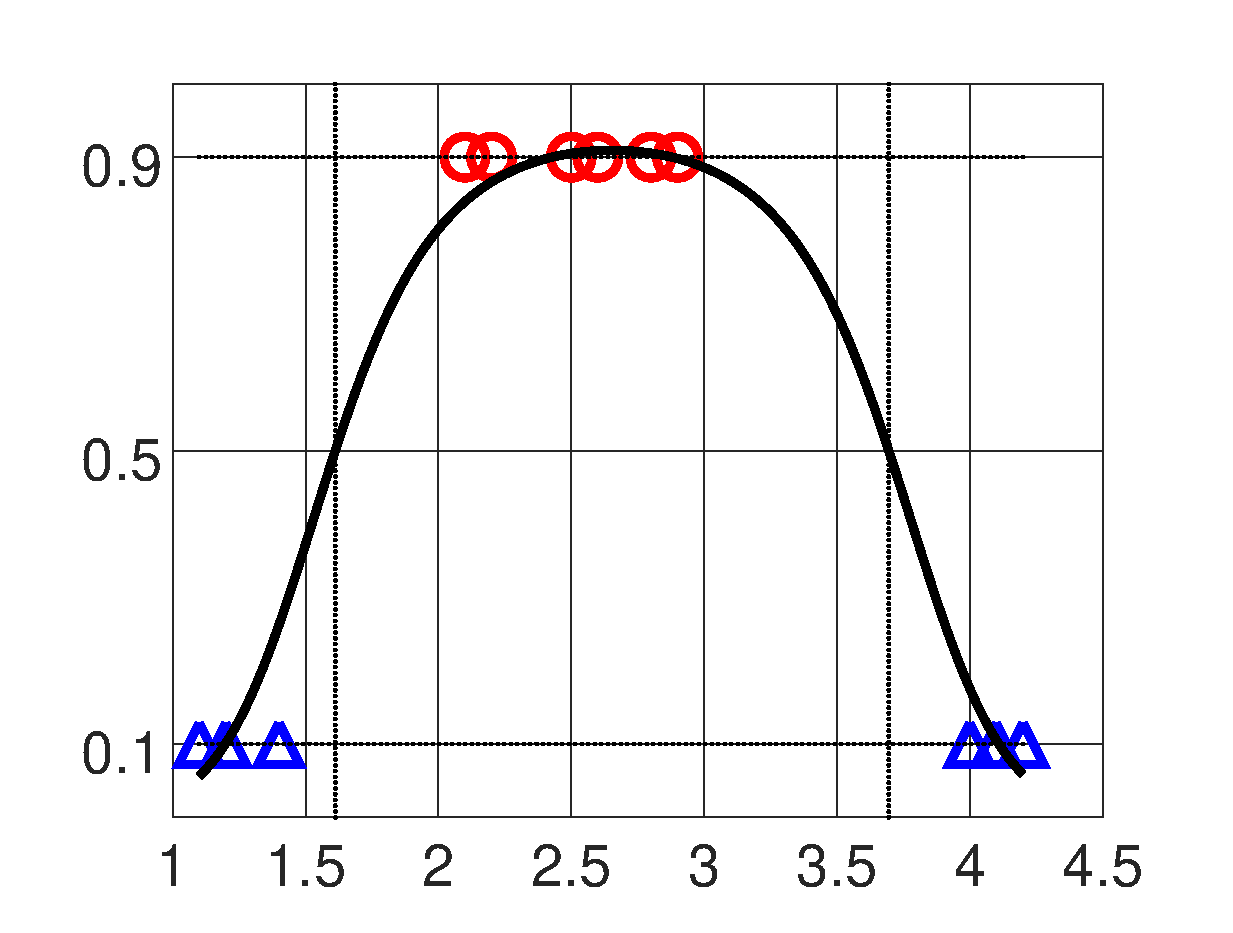
\includegraphics[width=\textwidth]{chapters/classificacao/mfiles/reglogr1r1poly/ex1s1-reglogr1r1poly.eps}
        \caption{Gráfico da classificação usando $y_l \in \{0.1,~ 0.9\}$.}
        \label{fig:theo:reglogr1r1poly:xn:s1}
    \end{subfigure}
    \hfill
    \begin{subfigure}[b]{0.45\textwidth}
        \centering
        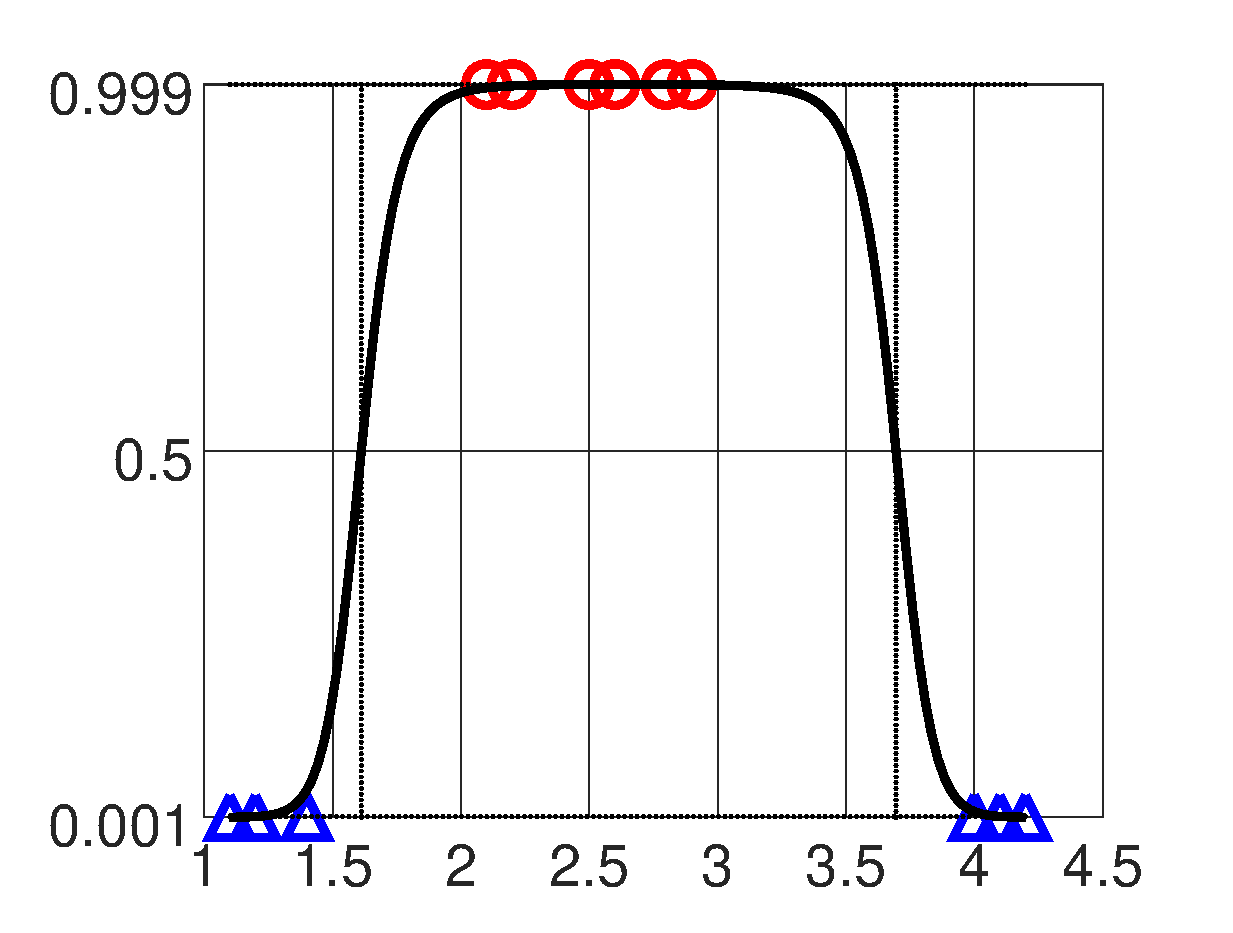
\includegraphics[width=\textwidth]{chapters/classificacao/mfiles/reglogr1r1poly/ex1s2-reglogr1r1poly.eps}
        \caption{Gráfico da classificação usando $y_l \in \{0.001,~ 0.999\}$.}
        \label{fig:theo:reglogr1r1poly:xn:s2}
    \end{subfigure}
    \caption{Classificação usando a função $f_{\VECTOR{c}}(x)$.}
    \label{fig:theo:reglogr1r1poly:xn}
\end{figure}


\begin{SolutionT}[Relativa ao Exemplo \ref{ex:theo:reglogr1r1poly}:]\label{sol:theo:reglogr1r1poly:s2}
Para obter o vetor de parâmetros $\VECTOR{c}=\VECTOR{\hat{c}}$ da função $f_{\VECTOR{c}}(x)$, 
que gere o menor erro $e(\VECTOR{c}) =  \frac{1}{L} \sum_{l=1}^{L} ||h_{\VECTOR{c}}(x_l)-logit(y_l)||^2$
com os $L=12$ dados $x_l$ da Tabela \ref{table:theo:reglogr1r1poly:xn},
usamos a Eq. (\ref{eq:reglogr1r1poly:2}) onde escolhemos $w_l=1$ e valores $y_l \in \{0.001,~ 0.999\}$,
$0.001$ para $\bigtriangleup$ e $0.999$ para $\bigcirc$,
obtendo um vetor $\VECTOR{\hat{c}}=[-39.8164\quad 35.4727\quad -6.6838]^{\transpose}$. 
Assim, podemos representar a função $f_{\VECTOR{c}}(x)$ que classifica os dados $x_l$, 
como é mostrado na Figura \ref{fig:theo:reglogr1r1poly:xn:s2} e na Eq. (\ref{eq:theo:reglogr1r1poly:xn:s2}),
\begin{equation}\label{eq:theo:reglogr1r1poly:xn:s2}
f_{\VECTOR{c}}(x)= \frac{1}{1+e^{-(-39.8164+35.4727 x -6.6838 x^2)}}.
\end{equation}
É interessante ressaltar que para um valor $A=0.001$ a pendente é abrupta para cada grupo com uma classificação bem definida,
e limiares de classificação em $1.6122$ e $3.6951$.
\end{SolutionT}
